\documentclass[11pt]{article}

\usepackage[a4paper,margin=0.9in]{geometry}
\usepackage{amsfonts}
\usepackage{amsmath}
\usepackage{amsthm}
\usepackage{cleveref}
\usepackage{ifthen}
\usepackage{rotating}
\usepackage{tikz}
\usepackage{caption}


\begin{document}
\author{Marco Milanta}
\title{Graded Homework 1, exercise 2}
\maketitle
% actually edit those files and create new sections if you need more. 

%% Special characters for number sets.
\newcommand{\N}{\mathbb{N}}


\newcommand{\R}{\mathbb{R}}
\newcommand{\E}{\mathbb{E}}

%% Vectors and sets.
\newcommand{\set}[1]{\mathcal #1}
\newcommand{\mat}[1]{\mathbf #1}
\renewcommand{\vec}[1]{\mathbf #1}
\newcommand{\x}{\mathbf{x}}
\newcommand{\w}{\mathbf{w}}
\newcommand{\X}{\mathcal{X}}
\newcommand{\D}{\mathcal{D}}
\newcommand{\ke}{\mathbf{k}}
\newcommand{\K}{\mathbf{K}}
\newcommand{\A}{\mathbf{A}}
\newcommand{\Y}{\mathbf{Y}}
\newcommand{\Si}{\Sigma}
%\newcommand{\Pr}{\mathbb{P}}

%% Bold greek letters.
\newcommand{\lm}{\boldsymbol{\lambda}}
\newcommand{\tht}{\boldsymbol{\theta}}
\newcommand{\ph}{\boldsymbol{\phi}}
\newcommand{\omg}{\boldsymbol{\omega}}

%% Theorems
\newtheorem{observation}{Observation}
\section*{Minimum Dominating Set in Special Graphs (15 points)}
We say that a graph is an \emph{$a$-forest} if the edges of the graph can be split into $a$ edge-disjoint forests. In each one of the forests we fix a root for each one of the trees, and orient the edges towards their parents in the trees. We say that $u$ is a \emph{parent} of $v$ if $u$ is a parent of $v$ in one of the $a$ forests. 

Recall that a set of vertices $D$ is a \emph{dominating set (DS)} of a graph $G$, if each vertex is either in $D$ or has a neighbor in $D$.
We say that a set of vertices $P$ is a \emph{parent-DS} of an $a$-forest graph $G$ if each vertex is either in $P$ or has a parent in $P$.

\begin{enumerate}
    \item Design an $O(a)$-approximation algorithm for finding a minimum size parent-DS in an $a$-forest graph $G$. The input to the graph is the $a$-forest, together with the orientation of the edges.
    \item Design an $O(a^2)$-approximation algorithm for finding a minimum size DS in an $a$-forest graph $G$. The input to the graph is the $a$-forest, together with the orientation of the edges. You can assume you have an algorithm for part 1 of the problem, even if you did not solve that part.
\end{enumerate}

\section*{Solution}
\begin{enumerate}
    \item\label{p:1} The algorithm will be found linking this problem to the one of minimum set cover with the maximum number of sets containing each element equal to $a$. Of course the link between the two problem is not trivial, we will divide it into steps. 
    
    We start with some definitions: let's denote the vertices of the graph as $e_1,\dots,e_n$. We define:
    \begin{align*}
        S_{i} &= \left\{e \in V \mid e_i = e \land \text{ or $e_i$ is a \textit{parent} of }e \right\}\qquad i \in 1:n,
    \end{align*}
    where with $1:n$ we indicate $1,\dots,n$. 
    \begin{observation}[Equivalence of problems] Let $\{e_{i_1},\dots, e_{i_m}\}$ be a parent-DS of an $a$-forest graph. Then $\{S_{i_1}, S_{i_{2}}, \dots, S_{i_{m}}\}$ is a collection of sets such that
        \begin{equation*}
            \bigcup_{j=1}^mS_{i_j} = V.
        \end{equation*}
    Where $V$ is the set of all vertices.
    \end{observation}
    \begin{proof}
        Given any vertice $e\in V$ there exists a $j\leq m$ such that either $e = e_{i_j}$ or $e_{i_j}$ is a parent of $e$. But this would imply that $e \in S_{i_j}$. We have then shown that all vertices are at least in one of the $S_{i_j}$, therefore they are in the union
    \end{proof}
    We have just shown that this problem is equivalent to the one of minimum set coverings with all the cost being set to $1$. We have a polynomial time algorithm to solve this problem with an $H_n$-approximation, but this is not good enough: we want an $O(a)$-approximation. For this we make another observation
    \begin{observation}[Elements in few sets] For any vertex $e_i$ there are at most $a+1$ different sets $S_j$ such that 
        \begin{equation*}
            e_i \in S_j.
        \end{equation*}
    \end{observation}
    \begin{proof}
        The proof simply follows from the fact that $e_i$ can have at most one parent per forest, he might have even less if it is a root in some forest. The total number of parents is no more than $a$. Finally, $e_i \in S_j$ only if $e_j$ is a parent of $e_i$ or $j=i$. Therefore, there are only $a+1$ acceptable sets. 
    \end{proof}
    In the case $a = 1$, then each element is contained by no more than $a+1 = 2$ sets. In this context we have shown in the lecture that there is an algorithm which yields a $2$-approximation. More generally, claim 1.9 from lecture notes gives us an $f$-approximation if every element is contained in at most $f$ sets. This would yield an $a+1$-approximation, which indeed is an $O(a)$-approximation. Once we have found the collection $\{S_{i_1}, S_{i_{2}}, \dots, S_{i_{m}}\}$ that minimizes the risk with our algorithm (in an $a+1$-approximation), we can easily get back to the solution of the original problem by taking $\{e_{i_1},\dots, e_{i_m}\}$ to be our parent-DS
    \item Here we use the same algorithm we used in part \ref{p:1}. We only need to show two more things: 
    \begin{itemize}
        \item The algorithm output is also a $DS$.
        \item The algorithm output is an $O(a^2)$-approximation of the minimum $DS$.
    \end{itemize}
    We know that the algorithm we use outputs a parent-DS. Now, in parent-DS each node is either inside the parent-DS or it has a parent in the parent-DS. Since the parents must be connected with an edge, it's easy to see that the parent-DS is also a DS.

    For the second point we define $OPT_{DS}$ to be the minimal dominating set, and $OPT_{pDS}$ to be the optimal parent dominating set.
    \begin{observation}\label{obs:extend}[Extend the DS] Given a graph $(V,E)$, with is $a$-forest. Let $OPT_{DS} \subseteq V$ be the minimal dominating set. Then there exists a $pDS \subseteq V$ such that $pDS$ is a parent-DS and
        \begin{equation*}
            \#pDS \leq (a+1) \# OPT_{DS}.
        \end{equation*}
    \end{observation} 
    
    Now, by calling $\mathcal{A}$ the outputs of our algorithm, we have that
    \begin{equation*}
        \#\mathcal{A} \stackrel{(i)}{\leq} (a+1)\# OPT_{pDS} \stackrel{(ii)}{\leq} (a+1) \#pDS \stackrel{(iii)}{\leq} (a+1)^2 \# OPT_{DS}.
    \end{equation*}
    Where $(i)$ follows from the approximation factor proven in part \ref{p:1}, $(ii)$ follows simply by the optimality of the solution of the parent-DS problem, and finally, $(iii)$ follows from observation \ref{obs:extend}. Then we can conclude that we have a $(a+1)^2 = O(a^2)$-approximation algorithm. The only thing left is to proof observation \ref{obs:extend}:
    \begin{proof}[Proof of observation \ref{obs:extend}]
        We start by $pDS = OPT_{DS}$, and we add some vertices to make it also a parent-DS. 
        
        
        Let $v$ be a vertex in $pDS$. Let $p_1, \dots, p_a$ be all of his parents (it might have less than $a$ parents, but this doesn't break the argument). And then $s_1,\dots,s_n$ be the set of sons (note that, in theory, a node could have as sons all $V$). By sons, we mean such vertices that have $v$ as parent.
\begin{figure}
        
            \begin{center}
        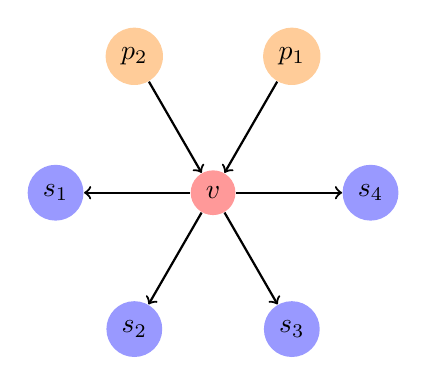
\begin{tikzpicture}
            
        \node[circle,fill=red!40] (n1) at (0,0) {$v$};

        \node[circle,fill=orange!40] (n2) at (-1,1.732) {$p_2$};
        \node[circle,fill=orange!40] (n3) at (1,1.732) {$p_1$};
        \node[circle,fill=blue!40] (n4) at (-2,0) {$s_1$};
        \node[circle,fill=blue!40] (n5) at (2,0) {$s_4$};
        \node[circle,fill=blue!40] (n6) at (-1,-1.732) {$s_2$};
        \node[circle,fill=blue!40] (n7) at (1,-1.732) {$s_3$};


        \draw[->, thick] (n2) -- (n1);
        \draw[->, thick] (n3) -- (n1);
        \draw[->, thick] (n1) -- (n4);
        \draw[->, thick] (n1) -- (n5);
        \draw[->, thick] (n1) -- (n6);
        \draw[->, thick] (n1) -- (n7);

    \end{tikzpicture}

    \captionsetup{width=.8\linewidth}
    \caption{The arrow indicates the parent-son relationship, the orange and the red together will compose $pDS$ in the end}\label{fig:n}
    \end{center}
\end{figure}
        Note that for each node $p_1,\dots,p_a,s_1,\dots,s_n$, which is the set of all sons and parents, is also the set of all the neighbors of $v$.

        Now, $pDS$, as a parent-covering, is not covering all of its parent, but he is still covering all of its sons. What we do is simply adding $p_1,\dots,p_a$ to $pDS$. Now, it's trivial that $pDS$ is parent-covering all the vertices in its neighborhood. Figure \ref{fig:n} might help with the intuition.

        Now we iterate this process (adding parents) for all vertices $v \in OPT_{DS}$. I would like to notice that $pDS$ is now a parent-DS, this is because it is parent-covering all the neighborhoods of all the vertices in $OPT_{DS}$. But $OPT_{DS}$ is a set covering, therefore the union of all the neighborhoods of all vertices of $OPT_{DS}$ is simply $V$.
        Finally, it's easy to see that at most we add $a$ vertices for any vertices in $OPT_{DS}$. Therefore
        \begin{equation*}
            \#pDS \leq (a+1) \# OPT_{DS}.
        \end{equation*}
    \end{proof}
\end{enumerate}
\end{document}